\problemname{Bingo}

Ture spelar en speciell sorts bingo som går till på följande sätt:
\begin{itemize}
\item Han har en kvadratisk bricka med $N$x$N$ rutor, vardera innehållande ett heltal. Samma tal kan finnas i flera rutor.
\item Spelledaren ropar ut ett godtyckligt heltal i taget. Om Ture har detta tal på sin bricka får han kryssa över det. Om han har talet i flera rutor måste han välja en enda ruta att kryssa över.
\item När Ture har kryssat en full rad med $N$ tal, antingen horisontellt, vertikalt eller diagonalt (se figur), så har han fått "bingo" och vinner en resa till BOI (Bingo Olympiad International).
\end{itemize}

Ture förlitar sig inte på turen utan har fuskat till sig den följd av tal som kommer att ropas ut. Skriv ett program som, givet Tures bricka samt följden av tal, beräknar efter hur många utrop Ture får bingo om han spelar optimalt.

\begin{figure}[!h]
\begin{center}
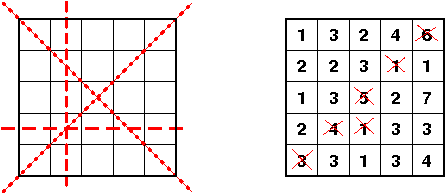
\includegraphics[width=0.6\textwidth]{bingo.png}
\end{center}
\caption{Vänster: De två diagonala raderna (prickade linjer) samt
  exempel på en horisontell och en vertikal rad (streckade
  linjer). Höger: Ett möjligt sätt att kryssa i det första exemplet.}
\end{figure}



\section*{Indata}
 
Första raden innehåller brickans dimension $N$, där $1\leq N \leq
100$, och antalet utrop $K$, där $1 \leq K \leq 10\,000$. Därefter följer $N$ rader vardera innehållande $N$ heltal i intervallet $1\ldots 1000$. Detta är Tures bingobricka. Slutligen följer en rad med $K$ heltal i samma intervall, de utropade talen i den ordning de ropas ut.

\section*{Utdata}

Ett heltal: det minsta antalet utrop som behövs innan Ture får en full rad (horisontellt, vertikalt eller diagonalt). Det kommer aldrig krävas mer än $K$ utrop.




